
\documentclass[12pt]{article}
\usepackage{geometry}
\geometry{a4paper}


\usepackage{color}
\usepackage{hyperref}
\usepackage{amsmath}
\usepackage{amsfonts}
\usepackage{amssymb}
\usepackage{graphicx}
\usepackage{tcolorbox}
\usepackage{listings}
\usepackage{here}
\usepackage{txfonts}
\usepackage{algorithm}
\usepackage{algorithmic}
\usepackage{siunitx}
\usepackage{xcolor}

\lstset {language = c++,
  basicstyle = \ttfamily \scriptsize,
  commentstyle = \textit,
  frame = tRBl,
  framesep = 5pt,
  showstringspaces = false,
  numbers = left,
  stepnumber = 1,
  numberstyle = \tiny,
  tabsize = 2,
  keywordstyle = \bfseries \color{blue},
  stringstyle=\color{magenta},
  commentstyle=\color{red},
  morecomment=[l][\color{red}]{\#}
  showstringspaces=false, % don't mark spaces in strings
}
\newcommand{\bi}[1]{\mathbf{#1}}
\newcommand{\bs}[1]{\boldsymbol{#1}}  % bold for greek characters
\newcommand{\bbR}{\mathbb{R}}

\author{Nobuyuki Umetani}


\title{Outline of Finite Element Method}
\author{Nobuyuki Umetani}

\begin{document}
\maketitle

\tableofcontents

\section{What is the Finite Element Method? }

Finite Element Method (FEM) is a method of finding a solution of \emph{partial differential equation in weak formulation} from \emph{mesh-based space spatially discretized field}.



\begin{figure}[htbp!]
\center
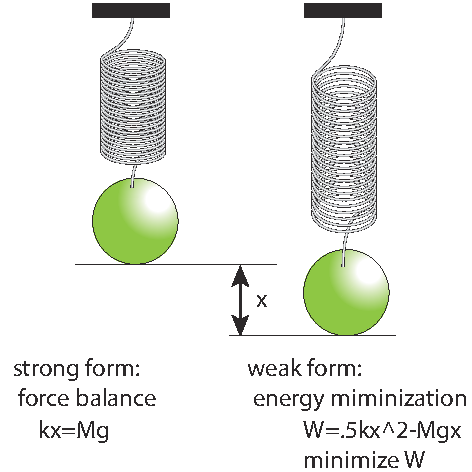
\includegraphics[width=80mm]{images/spring.pdf}
\caption{Difference between strong formulation and weak formulation.}
\label{fig:spring}
\end{figure}

\paragraph{Weak formulation} Imagine a spring.  Weak: energy based. global energy minimization Strong:micro equilibrium. 
%
Key element of the FEM is how we can transform a strong formulation into a weak formulation.


\begin{figure}[htbp!]
\center
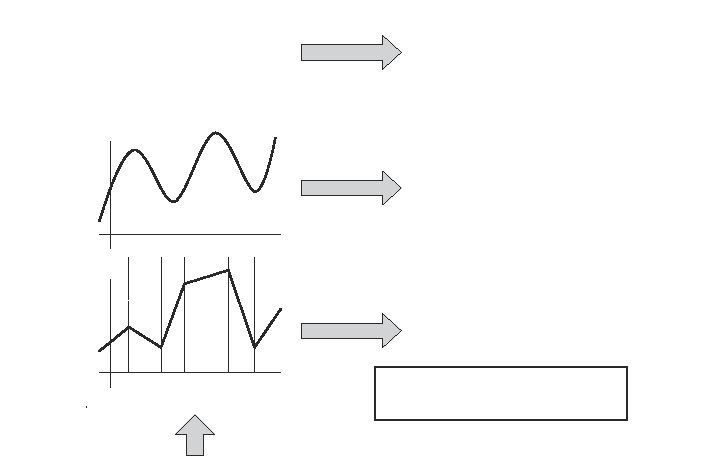
\includegraphics[width=120mm]{images/fem_variational_overview.pdf}
\end{figure}




\subsection{Discretizing Field using Mesh}
A physical ordinary field has an infinite dimension, but since computers can not represent infinite dimensional fields, of course, on a computer, we express the field with a finite number of values. This is why it is called ``finite" element method. 
%
Let's see how to express the field using finite variables.
%
The mesh is used for the data representation (finite element method interpolation field) of the field by the finite element method. 
%
The mesh is obtained by dividing the analysis region with a simple polygon (triangle or quadrangle in the case of two dimensions, tetrahedron, hexahedron in case of three dimensions). 
%
Finite Element Method The interpolated field is made up of a set of nodal arrays and element arrays.
%
A node is a point in space and has a value of a field at that point. 
%
A nodal array is an array in which the coordinates of a node and the value of a field (temperature, displacement, etc.) are aligned.


\begin{figure}[htbp!]
\center
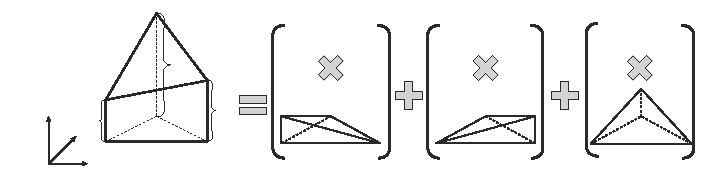
\includegraphics[width=120mm]{images/triangle_interp.pdf}
\label{fig:triangle_interp}
\end{figure}


I do not know how the field other than the node is with nodes alone. 
%
I will use elements there. 
%
An element is a polygon in the mesh and has information on which node the element has, which is essentially a collection of nodal indexes. 
%
Interior elements are interpolated using interpolation function.




Since nodes are shared between adjacent elements, the field is never discontinuous ($C^0$ grade). The mesh is made to fill all the analysis areas. So, one point in the analysis area should always be on a certain element or on its boundary. You can find the value of an arbitrary point in the analysis area by finding the interpolation in the element that contains the point or on the side. Since continuous interpolation is used within the element and its boundary, we can see that this field is continuous.

\subsubsection{example of mesh}
The element array of the mesh as shown below is as follows.
%
\begin{figure}[htbp!]
\centering
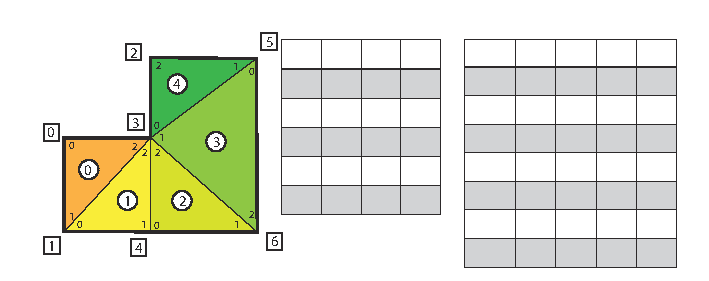
\includegraphics[width=120mm]{images/fem_data.pdf}
\end{figure}








\section{Weakly formulated partial differential equations}
%
The weak form is an extension that makes it possible to obtain solutions in a wider range of partial differential equations. 
%
In the strong form, two times can be differentiated consecutively ($C^2$ grade), but quite strong smoothness was required, but in the weak form, it suffices if weak derivative of the first floor is integrable ($H^1$ grade), it is quite wide solutions can be taken in the range. 
%
Mesh represented field is often impossible to differentiate at the connecting part of the element. For example, one-dimensional temporary interpolation is a polygonal line (piecewise linear function), so differentiation there is not defined. But weak differentiation can also differentiate such a function. If a strong format solution exists, it is also a weak form solution (weak solution). The weak form is a natural extension of strong form.
%
Another important thing in weak form is that it is a variational form and is written in the form of integral. 
%
Integration is an operation like addition in the region, since the analysis region is filled with elements, the integral value of the whole region can be obtained by adding the integral value for each element. Since each element has a simple shape, integration within an element can be easily done numerically and analytically. 
%
Integrating is an important function of the mesh as well as creating an interpolation field.


\subsection{Example of weak formalization of Poisson equation}
Taking a Poisson equation as an example, let's try weak formalization.
%
\begin{eqnarray}
\left\{\begin{array}{rll}
-\nabla\cdot( \nabla \phi) &=& f\;\;in\;\Omega\\\ 
\phi&=&0\;\;on\;\partial\Omega
\end{array}\right.
\end{eqnarray}

By multiplying the strong form above by $\delta\phi \;\; (\delta\phi=0\;\;on\;\partial\Omega)$, integrating in the region and then using the Green-Gauss formula, we can convert it to the following weak form.

\begin{equation}
\int_{\Omega} \nabla\delta\phi\cdot\nabla\phi d\Omega = \int_{\Omega}\delta\phi f d\Omega
\end{equation}


Many problems of the finite element method can be written using $\bi{f}$ (according to Riesz 's expression theorem) which is a conjugate space to the space to which $\phi$ belongs and $\bi{a}$ of bilinear form as follows.
\begin{equation}
\bi{a}(\delta\phi,\phi)=\delta\phi\cdot f\;\;\;\forall \delta\phi
\end{equation}

This is a potential
\begin{equation}
\bi{W}(\phi)=\frac{1}{2}a(\phi,\phi)+f\cdot\phi,
\end{equation}

It means that the extreme value of the potential is a solution.
\begin{equation}
find\;\phi\;s.t.\;\delta\bi{W}=0
\end{equation}

$a$ has the property as a norm and this is called the energy norm. Furthermore, we can see that there is only weakness due to the nature such as the compatibility and boundedness of the operator $a$. 
%
Therefore, we can see that the solution is the minimum potential value.
%
\begin{equation}
find\;\phi\;s.t.\;minimize\; W
\end{equation}

This potential is usually the same as energy when solving a physical problem. For example, the potential in solid dynamics analysis represents strain energy. The potential in electromagnetic also represents the energy of the electromagnetic field. The fact that the potential is minimal is the same as the principle of energy minimization. format





\section{Creating Linear System from Weak From Partial Differential Equations by Finite Element Discretization}
%
Now, let's substitute a finite element method interpolation field for weakly formalized partial differential equations to create simultaneous linear equations. 
%
Let's assume that $\phi,\delta\phi$ is expressed by the sum of the product of the value $\phi^b,\delta\phi^a$ at the node and the basis function $N^a,N^b$ of the field as follows.
%
\begin{equation}
\phi = N^b\phi^b,\;\;\;\delta\phi = N^a\phi^a
\end{equation}

Substituting this into the previous formula yields a simultaneous linear equation to solve.
%
\begin{eqnarray}
&& a(N^a\delta\phi^a,N^b\phi^b)=(N^a\delta\phi^a)\cdot\bi{f}\;\;\;\forall \delta\phi^a\\
&\Leftrightarrow& \delta\phi^a a(N^a,N^b)\phi^b = \delta\phi^a(N^a\cdot\bi{f})\;\;\;\forall \delta\phi^a\\
&\Leftrightarrow& a(N^a,N^b)\phi^b = (N^a\cdot\bi{f})\\
&\Leftrightarrow& A^{ab}\phi^b = f^a\;\;\;\;(where,\;\;A^{ab}=a(N^a,N^b),\;f^a=N^a\cdot\bi{f})
\end{eqnarray}

Solve the simultaneous linear equations obtained to get a solution.
Calculation of the component $A^{ab}=a(N^a,N^b)$ of the actual coefficient matrix is ​​done for each element and made by adding them together.
Let's take a look at the Poisson equation for this calculation.


\subsection{Integration of element units seen in Poisson equation}
The weakly formatted Poisson equation was as follows.
%
\begin{equation}
\int_{\Omega} \nabla\delta\phi\cdot\nabla\phi d\Omega = \int_{\Omega}\delta\phi f d\Omega
\end{equation}

The calculation of the integral is the addition of things done for each element.
%
\begin{equation}
\sum_e^n\int_{\Omega_e} \nabla\delta\phi\cdot\nabla\phi d\Omega = \sum_e^n\int_{\Omega_e}\delta\phi f d\Omega
\end{equation}

\begin{figure}[htbp!]
\center
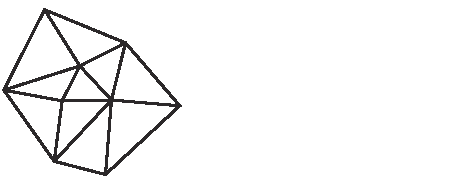
\includegraphics[width=120mm]{images/variational_integration.pdf}
\label{fig:variational_integration}
\end{figure}


Let's assume that in an element $\phi,\delta\phi$ is expressed by the sum of the product of the value $\phi^q,\delta\phi^p$ at the node and the basis function $N^q,N^p$ of the field as follows:
%
\begin{equation}
\phi = N^q\phi^q,\;\;\;\delta\phi = N^p\phi^p
\end{equation}

Also assume that the numbering $\{p,q\}$ in the element corresponds to the node numbering $\{a,b\}$. When this is substituted, the above expression becomes as follows.

\begin{eqnarray}
&&\sum_e^n\int_{\Omega_e} \nabla (N^p\delta\phi^p)\cdot \nabla (N^q\phi^q ) d\Omega = \sum_e^n\int_{\Omega_e}(N^p\delta\phi^p) f d\Omega\;\;\;\forall\delta\phi^p\\
&\Leftrightarrow& \sum_e^n\delta\phi^p\int_{\Omega_e}\nabla N^p\cdot\nabla N^q d\Omega \phi^q = \sum_e^n\delta\phi^p\int_{\Omega_e}N^p f d\Omega\;\;\;\forall \delta\phi^p\\
&\Leftrightarrow& \delta\phi^a\sum_e^n \left(A_e^{pq}\right)\phi^b=\delta\phi^a\sum_e^n f_e^p\phi^a\;\;\;\forall \delta\phi^p\\
&\Leftrightarrow& \sum_e^n \left(A_e^{pq}\right)\phi^b=\sum_e^n f_e^p
\end{eqnarray}

here

\begin{equation}
A_e^{pq}=\int_{\Omega_e}\nabla N^p\cdot\nabla N^q d\Omega
\end{equation}

Is called the element stiffness matrix. Compared to the previous equation, we can see that the total stiffness matrix $A^{ab}$ is this sum. When adding together, use the numbering of the nodes in the element and the correspondence of the node numbers. $A_e^{pq}$ is added to $A^{ab}$ since $\{p,q\}$ corresponds to the numbering of $\{a,b\}$ of the entire node now, numbering the nodes in the element. Such a process of adding is called ``Marge".

The solution (weakness) of the weakly formulated equation is found to be a solution that minimizes the energy norm in a certain space (subspace of $H^1$ space that satisfies the boundary condition in most problems) It was.
In the $H^1$ space, a solution that minimizes the energy norm in the finite element method interpolation field, which is its subspace, is a solution in the finite element method.
When the interpolation function and the test function are the same space, numbering It is called the Galerkin method.
In the Galerkin method, we can see that it is also a solution that appears in a finite element method interpolation field that is closest to the weak solution in the energy norm.
However, in the absence of energy like a fluid, a more accurate solution may be obtained by selecting the interpolation function and the test function from different spaces.


\if0
\section{Procedure of Finite Element Method Analysis}
Below is the overall flow of finite element analysis.
CENTER: file: fem_algorithm.jpg
CENTER: & bold (flow of finite element method);
The pseudocode of the finite element method is as follows.
 // pseudocode of the finite element method procedure

 ? Create a model
 ? Generate a mesh
 ? Create a finite element method interpolation field
 do i = 1, number of elements
 ? Retrieve the node data referenced by the element
 ? Integrate weakly formulated governing equation per element
 ? Add the stiffness matrix and the residual vector per element obtained by integration to the whole.
 end do
 ? Solve simultaneous linear equations consisting of total rigidity matrix and residual vector to obtain an update vector
 ? Update the solution using the update vector.
 Visualize the field
\fi

\end{document}
